\chapter{Algoritam Sparc}

Cilj ovog projekta bio je implementirati algoritam Sparc \citep{ye2016sparc} koji se koristi u konsenzus fazi preklapanje-razmještanje-konsenzus (engl. Overlap-Layout-Consensus, OLC) pristupa.
Sparc je algoritam za konsenzus fazu OLC pristupa, temeljen na \emph{k-mer/de Bruijn} \citep{hannenhalli1996positional} grafovima.

\section{Ulaz u algoritam}
TODO: seke
Algoritam koristi izlaz iz faze razmještanja OLC pristupa te sva početna očitanja genoma.
Očitanja su mapirana na kontigu iz faze razmještanja i pohranjena u datoteku formata .sam, opisanom u nastavku.

Kako bi uspješno izgradili graf i proveli algoritam, potrebno je znati gdje se pojedina očitanja mapiraju na osnovnu kontigu.
Te informacije dobivano iz .sam datoteke koju smo generirali alatom \emph{GraphMap} \citep{sovic2016fast}.
Nama najvažnije informacije u datoteci jesu:
\begin{description}
  \item [POS] pozicija na osnovnoj kontizi na kojoj počinje mapiranje pojedinog očitanja
  \item [CIGAR] operacije obavljene nad očitanjem kako bi se dobilo mapiranje (dodavanje, brisanje, pomicanje, itd.)
  \item SEQ: očitana sekvenca u prvotnom obliku (bez obavljenih CIGAR operacija)
  \item [QUAL] kvaliteta očitanja (iz .fastq datoteke očitanja)
\end{description}

Važnost navedenih informacija bit će jasnija kasnije.
Za naše potrebe, spremili smo sve važne informacije u zasebnu datoteku koja se sastoji od osnovne kontige (engl. backbone, layout) u prvoj liniji.
U nastavku datoteke su očitanja zapisana kroz tri linije.
Prva linija predstavlja originalno očitanje na koje su primjenjene CIGAR operacije kako bi se dobilo poravnanje s backbone-om.
U drugoj liniji nalazi se kvaliteta očitanja (QUAL), a u trećoj je pozicija na backbone-u na kojoj počinje mapiranje izmjenjene sekvence.

\section{Opis algoritma}
TODO: paljak
Najprije se gradi graf direktno iz backbone-a, kako je prikazano na slici \ref{fig:sparc.png}.
Linearno se prolazi kroz backbone te se u čvorove stavljaju \emph{k-torke (k-meri)}, a bridovi su definirani kao postojeći, ako su sufiks jednog čvora, a prefiks drugoga. 
Zatim se prolazi kroz mapirana očitanja te se ažuriraju težine u grafu gdje dolazi do preklapanja.
Dodaju se novi čvorovi i bridovi ako se u očitanju javljaju nove k-torke.
Konačni korak je pronalazak najtežeg puta u grafu.
Primjer izgradnje grafa dan je na slici \ref{fig:sparc}.
TODO: objasni bolje

\begin{figure}[htb]
\centering
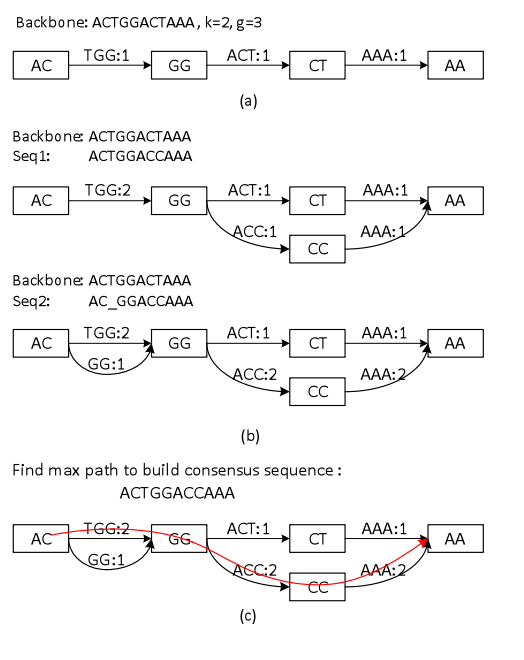
\includegraphics[scale=0.6]{figures/sparc.png}
\caption{Izgradnja grafa.}
\label{fig:sparc}
\end{figure}

